\section{Existing solutions}\label{sec:exist}

During the early stages of the project we began searching for existing solutions to draw inspiration to the design and implementation phases. All members of the group have previously had experience using different recipe sites on the Internet, and we think that the existing solutions lack functionality. In this section we review and discuss the existing solutions and draw some good practices from these.

\subsection{Supercook}
Supercook\cite{supercook} is a website with focus on searching for recipes based on their ingredients, however you can also search for recipes using free-text. 

When searching using ingredients the user is limited to enter a set of ingredients which is defined by Supercook. When adding ingredients to a search the user is aided by autocompletion and a word cloud with ingredients.

The word cloud changes according to the type of ingredients you have entered, e.g. if you enter ``vanilla'' the word cloud will change to contain, typical, cake ingredients. It is possible to apply restrictions to your search, e.g. ``I don't eat meat'' and all recipes with meat will be excluded. A search on Supercook will result in a prioritised list of links to recipes from several online cookbooks. A screenshot of the website is shown in \autoref{fig:supercook}.

\begin{figure}[H]
\centering
\fbox{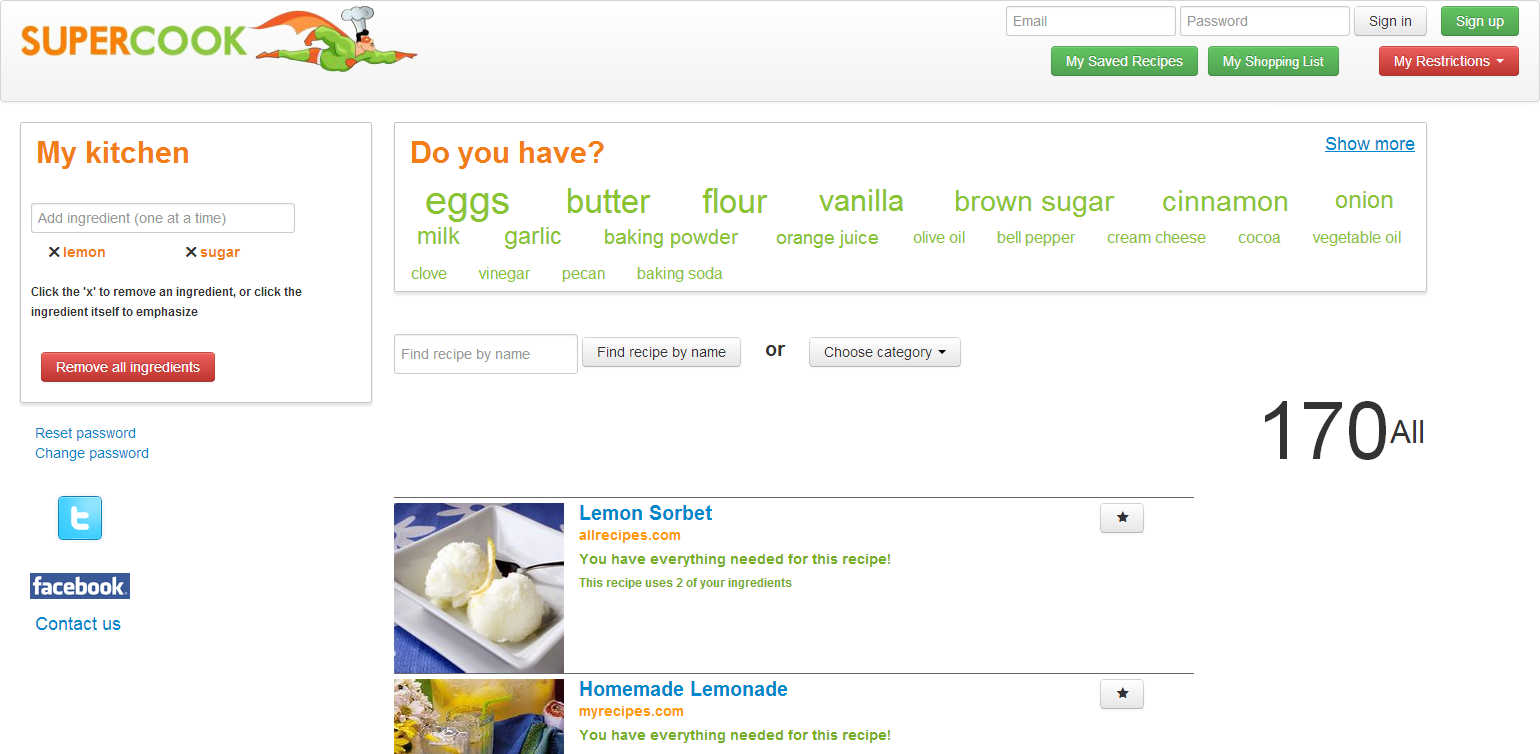
\includegraphics[width=\linewidth]{img/screenshots/supercook.png}}
\caption{The inferface of Supercook.}
\label{fig:supercook}
\end{figure}

By evaluating the search results of Supercook, we have deduced what we believe are the precedence function used to generate the search results:
\begin{enumerate}
	\item Remove recipes without any matching ingredients.
	\item Sort by most matching ingredients.
	\item Sort by least missing ingredients.
\end{enumerate}
We have also noticed some quirks in the way it counts matching ingredients. It seems like the search algorithm counts the number of occurrences of the entered ingredients in the recipes. When entering ``bell pepper'' and ``olive oil'', recipes which contain both red, green, and yellow pepper are prioritised higher than recipes which actually contains both of the entered ingredients. It also appears as if ingredients in the recipes are mapped to the ingredients defined by Supercook. An example of that is that ``flour'' appear to be mapped to ``flour'', ``wheat'', ``oat'', etc. This also appears to have the shortcoming that recipes containing e.g. ``wheat flour'' are prioritised as if they have two matching ingredient when the user entered ``flour'', since Supercook detect both ``wheat'' and ``flour''.

When making a search containing ``eggs'', ``garlic'', ``ground beef'', and ``onion'', we get a result which showcases a drawback of the sorting done by Supercook. The first 94 recipes are simple recipes using only few of the entered ingredients, including 24 recipes on how to boil an egg. Recipe number 95 is a recipe for meatballs and is using all entered ingredients but it also needs ``bread crumbs''. The reason why the first 94 recipes are prioritised highest is because they do not need any other ingredients than the ingredients entered.

\subsection{Allthecooks}
Allthecooks is one of the most downloaded \cite{allthecooks-googleplay} Android applications that is related to the search: ``recipe''. The application design follows the Android guidelines\cite{guidelines-appstructure}\todo{Vi skal finde ud af had vi gør med det her Android Guidelines} which makes it intuitive and easy to navigate. The detailed display of a recipe is especially well implemented, the user has everything on a single page, and can easily see the needed ingredients and the required steps to cook the recipe. The user can also, by a press of a button, toggle between different measuring units, or add the selected ingredient to a shopping list. Screenshots of the application are shown in \autoref{fig:allthecooks-menu}, \ref{fig:allthecooks-detail1}, \ref{fig:allthecooks-detail2}, and \ref{fig:allthecooks-detail3}.

The recipes of Allthecooks are user created, meaning they are created and uploaded by users. The photos are also provided by users, this can be dangerous if the photos are not checked for content not suitable for the application's audience. An advantage of user created recipes is that the applications content is growing with the audience of the application.
The search is free-text based, which means that opposite the Supercook web application it is hard to find recipes based on ingredients. You are able to apply filters to your search to remove recipes that contain certain ingredients.\todo{det var vist ikke helt rigtigt at supercook ikke have free-text}
\twofigs{screenshots/menu.png}{Menu of Allthecooks}{fig:allthecooks-menu}{screenshots/rainbowcake-1.png}{Detail display of a recipe}{fig:allthecooks-detail1}
\twofigs{screenshots/rainbowcake-2.png}{Buttons for different features}{fig:allthecooks-detail2}{screenshots/rainbowcake-3.png}{Directions for the recipe}{fig:allthecooks-detail3}

\subsection{BigOven}
BigOven is also one of the most downloaded \cite{bigoven-googleplay} Android application that is related to ``recipe''. The application's navigation and design does not follow the Android guidelines\cite{guidelines-appstructure}\todo{Igen med guidelines} and therefore the application's navigation can be quite confusing to an Android user.

The application main page is cluttered and presents the user with many functionalities, see \autoref{fig:mainpage-bigoven}. It is possible to search both by ingredients and free-text. The search by ingredients is limited to only three ingredients and the algorithm finds only the recipes where they all are included. The search by ingredient is based on free-text, meaning the user does not have the aid of autocompletion, like with Supercook. If the user inputs three ingredients that have no real relation like: ``beef'', ``cake-mix'', ``salmon'', the search by ingredients would find no results, the search by ingredients excludes everything that does not contain all three ingredients. Like Allthecooks the user can add the different ingredients to a shopping list, save the recipe to favourites, and alternate between the metric and imperial system.

A cool feature that is unique to the BigOven application is the menu-cards, see \autoref{fig:menucards-bigoven}.
\twofigs{screenshots/mainpage-bigoven.png}{The main page of BigOven}{fig:mainpage-bigoven}{screenshots/menucards-bigoven.png}{Menu Cards from BigOven}{fig:menucards-bigoven}
It is a small collection of different recipes that together builds to a meal, e.g. ``steak'', ``fries'', and ``green beans''. Each meal is bound to a day, which means that the user can create a menu-card that can contain a meal for each day of the week, or more. 

The recipes of BigOven is also, like Allthecooks, user created, which provides the same risks and benefits as explained in the previous section.
The BigOven application is free, but you can buy Pro-features that exclude advertisers from the application and unlocks more functionality in the application.

\subsection{Comparison}
These three applications have been chosen for comparison since they vary in focus, design, navigation, and features. Allthecooks focus on design and navigation, where as BigOven has focus on features. Supercook is a bit different since it is not an Android application, but it was included in the comparison since it had a unique set of features, such as the word cloud, and search by ingredients.
Allthecooks and BigOven share a lot of features, they both have free-text search, shopping list, and saving of recipes. Though BigOven has some features that are unique, such as search by ingredients, and menu-cards. A noticeable thing about BigOven is that the experience of using the application could be improved significantly, both in its design and performance.

BigOven and Supercook is both able to search by ingredients, but there is a big difference in the two searches. In the BigOven application you are only able to enter three ingredients, the search finds all the recipes that include all three ingredients. BigOven also uses free-text as an input method, whereas Supercook aids the user with autocompletion. In Supercook the user is also able to enter as many ingredients as necessary.
A comparison between the existing solutions can be seen in \ref{tab:appcomparison}.
\begin{table}[H]
\centering
\begin{tabular}{|>{\bfseries}l|l|l|l|}
\hline
 & \textbf{Supercook} & \textbf{Allthecooks} & \textbf{BigOven} \\
\hline
Platform & Website & Android/Website & Android/Website \\
\hline
Cost & Free & Free & Free \& Paid \\
\hline
Recipe search & Yes & Yes & Yes  \\
\hline
Ingredient search & Yes & No & Yes \\
\hline
Recipe origin & Web crawl & User defined & User defined \\
\hline
Shopping list & Yes & Yes & Yes \\
\hline
Menu planner & No & Yes & Yes \\
\hline
Saving recipes & Yes & Yes & Yes \\
\hline
Ingredient filter & Yes & Yes & Yes \\
\hline
Sharing of shopping list & No & E-mail/SMS & E-mail \\
\hline
Sharing of recipe & No & App/SMS/E-mail & App/E-mail \\
\hline
Needs Internet & Yes & Yes/No & Yes \\
\hline
Needs login & No & No & No \\
\hline
\end{tabular}
\caption{Application comparison}
\label{tab:appcomparison}
\end{table}
The user does not need to be signed in to search for recipes in any of the applications. 
In BigOven the user needs to be signed in to save recipes to favourites and adding item to the shopping list. 
In Allthecooks the user does not need to be signed in to save recipes to favourites, but the user still needs to be signed in to access the shopping list.  
In all applications you need Internet to search and access the recipes, they are not stored locally on the device, though in the Allthecooks the user are able to view its favourites and shopping list without a Internet connection.

